\section{Consensus}

\subsection{Diagrams}

\begin{figure}[H]
    \centering
    %\includegraphics[width=4.11in,height=5.0in]{media/image15.jpg}
    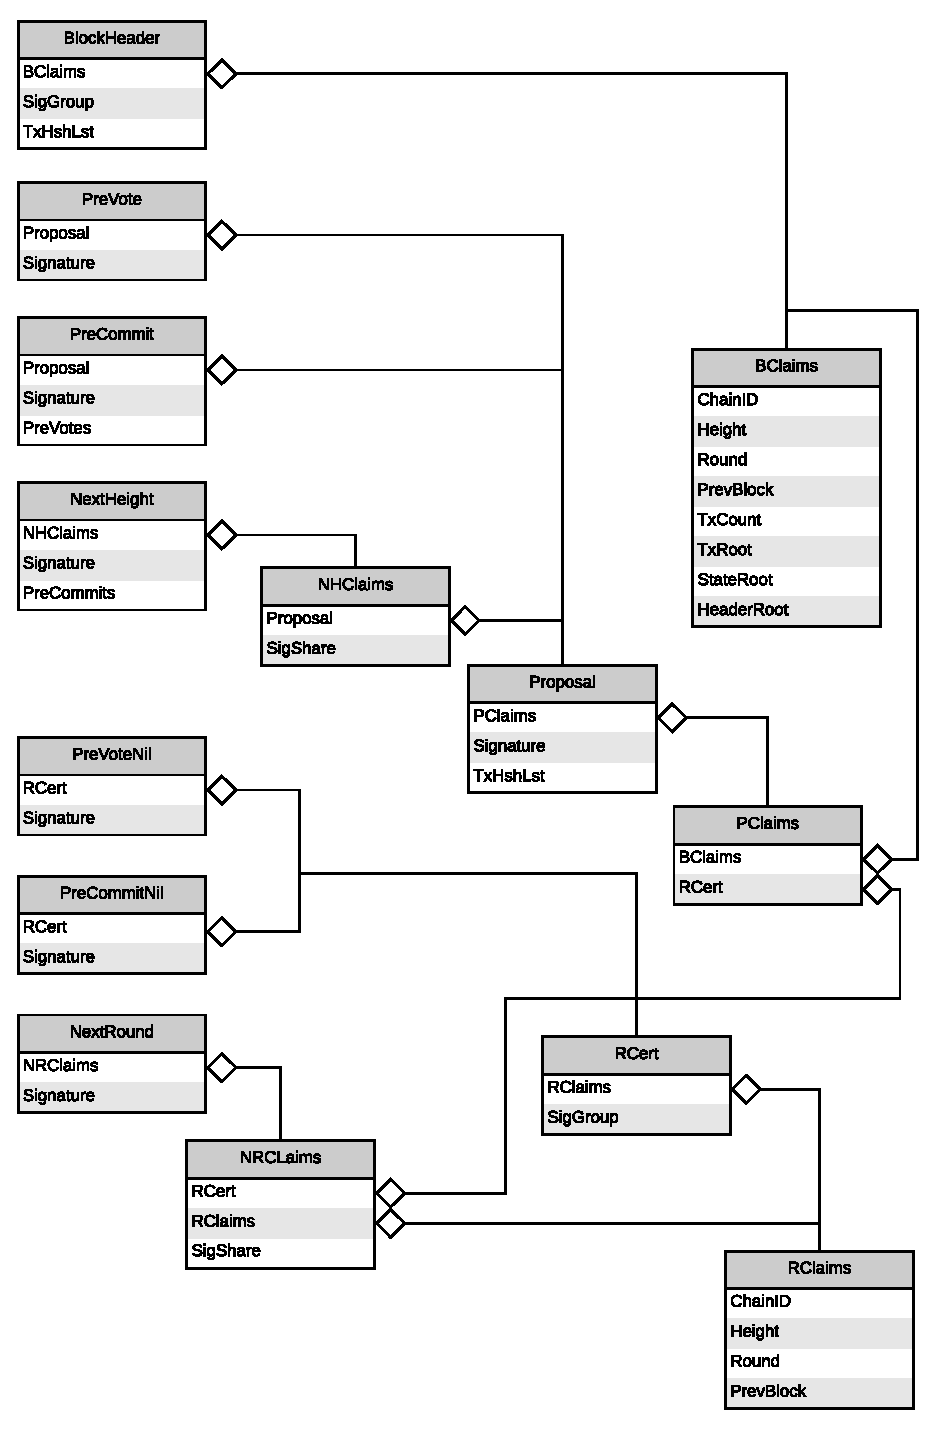
\includegraphics[scale=0.5]{figures/Consensus_Object_Primitive.pdf}
    \caption{Consensus Object Primitives}
\end{figure}



\subsection{Definitions}

\begin{labeling}{BlockHash}
\item [Validator] A validator is a node that has placed a stake in the
    Ethereum staking smart contract, successfully negotiated a group key,
    and is actively participating in block creation on MadNetwork.
    Validators coordinate the generation of new blocks through a
    Byzantine Fault Tolerant consensus algorithm.
\item [Height]
    The number of blocks that are in the blockchain starting from index one.
\item [BlockHash] A cryptographic hash of the canonical encoding
    of the BClaims object.
\item [ChainID] A unique uint32 value used to identify a particular
    instantiation of the MadNetwork blockchain software.
\item [Round] A round is defined by an iteration of the consensus
    protocol in which a single validator may be considered the leader.
    For each change of leader that occurs without a new block being
    produced, the round is incremented.
    The round starts at index one and is monotonically increasing.
    Upon a new block being produced, the round is reset to one.
\item [SigShare] This is a signature of an object under a BLS threshold
    cryptosystem.
\item [SigGroup] This is the aggregated signature formed by a threshold
    number of SigShares.
\item [Signature] Signatures are validator signatures under the
    secp256k1 curve using the Ethereum compliant recoverable ECDSA algorithm.
\end{labeling}


\subsection{Cryptography}

We use Elliptic Curve Cryptography within our system.
Specifically, we use the curves Secp256k1 and BN256-Eth.
Secp256k1 is the same elliptic curve used by Bitcoin and Ethereum
for their public key cryptography.
BN256-Eth is the pairing-friendly elliptic curve from the Ethereum
blockchain which is convenient for constructing group signatures.
All validators are required to have an Ethereum account and so they
have a Secp256k1 public key.
During the distributed key generation process, a master public key (a
public key for the entire group) is constructed and split amongst the
participants.
Each member is able to compute a partial signature, and these partial
signatures are able to be combined into a group signature.
A more in-depth discussion about cryptography is relegated to
Appendix~\ref{sec:tech_crypto}.


\subsection{Storage and Data Persistence}

In order to ensure all information is stored in a system that is
efficient, crash resilient, and allows transactional updates, BadgerDB
was selected as the backing storage mechanism for the system.
The consensus mechanism may be built on other key value stores in a
similar manner, but the choice of Golang as our programming language
made BadgerDB an optimal choice for an embedded key value store.
BadgerDB also supports PubSub systems, allows namespacing of objects
through key prefixes, ordered/key only iteration, and many other useful
primitives.

In the context of the consensus algorithm, the crash resilience and
PubSub mechanisms have been leveraged to simplify the problems
surrounding accidental violations of validator protocol.
These accidental violations are most likely to occur in other systems
when a crash occurs as a value is being written to a database and also
being transmitted to peers.
Such crash conditions could allow an otherwise honest party to act in a
contradictory manner through nothing more than a crash problem coupled
to a race condition.
In order to mitigate such problems, we leverage the PubSub system of
BadgerDB to send messages out to peers only after they have been
verified as having been flushed to the file system.
This decoupling also allows the simplification of the consensus
algorithm logic by not requiring complex locking and chaining of
operations.

Future versions of the node software will include the ability to
coordinate data persistence in a master slave failover architecture for
validator nodes.
This will mitigate the previously described race condition under the
extended assumption that multiple validators are being run in a
failover configuration and both validators use the same signing key.
This race condition caused the first slashing event on the Cosmos Hub,
so it is worth addressing.
Fortunately the same PubSub system may be leveraged to facilitate this
action painlessly.
This may be implemented by forcing the master to write each message to
the database at a location that causes the PubSub system to send a
message to the slave.
The system may then wait for an ack response from the slave that
specifies the key of the value that has been persisted to disk.
Another thread in the master process may then write this same value to
a location that is monitored by the PubSub system for transmission as
gossip to other peers.
Through this simple modification a single master slave configuration
may be built that ensures atomic coordination between the master and
slave while sacrificing a small latency in network operation.


\subsection{Protocol Overview}

The MadNetwork consensus protocol is based on a modified form of
Tendermint.
In our implementation we utilize the PaceMaker concept of HotStuff in
order to create stronger bounds on the mean time to consensus.
This is implemented as the RCert system described below.
Unlike Tendermint, we do not allow transitions between rounds to occur
as the default response to a timeout.
In order to exit a round, the system requires at least threshold
messages have been observed in each intermediate state.
A validator may also exit a round or height, with constraints, if a
proof of consensus is observed for a higher round/block.
The observation of these threshold messages allows the formation of a
group signature under a threshold signature scheme.
This leaves the potential for halting problems to arise under double
proposing in a round, but we have addressed the halting problems
through a novel concept we have named virtual voting.
The flow of this protocol is also optimized through an optimistic fast
path that allows termination of the protocol in slightly more than a
single timeout under general consensus.
The system does, however, force slower operation under split votes in
order for more state information to be observed before forward progress
is made.

This system is operated as a Proof of Stake sidechain to the Ethereum
Blockchain.
This network is governed and secured through the use of smart contracts
that exist in the Ethereum Blockchain.
This choice of operations allows the system progress to be governed by
a system that is beyond the control of the validators in the Proof of
Stake protocol itself.
Thus, many complexities around malicious majority attacks may be
mitigated either completely or at least in part.

The system operates on a hierarchical division of time.
The measurement of this time is relative to two systems.
The first system is the Ethereum blockchain.
The system protects some actions from occurring until a threshold
number of blocks have occurred in the Ethereum blockchain to prevent
attacks that attempt to violate required delays of the system through
pre-arranged message negotiation in secret.
The full details of these attacks are not covered because they have
been mitigated, but the basis for these attacks is apparent in the
section describing validator stake withdrawal operations.

The second system of time measurement is local blocks within the Mad
Network itself.
Large groups of these blocks form Epochs.
An epoch is defined for two purposes.
First, it designates a boundary point for recording a snapshot of
blockchain state into an Ethereum smart contract.
Second, it provides a logical transition point for the exit and
entrance of new validators.

In order to build the protocol in an auditable manner, a synchronous
core algorithm was designed such that asynchronous messages may be
queued for processing.
The primary control loop for the consensus algorithm is a three state
system.
The system begins in the unsynchronized state.
Once synchronization is complete, the algorithm alternates between
updating local state based on messages observed and collecting messages
for processing and storage.

All network interaction is decoupled from the consensus algorithm
proper through the use of BadgerDB's native PubSub mechanisms.
Thus, a message may never be placed on the wire without first being
recorded in the database.
In the following explanation network communication should be assumed to
occur following writes to persistent storage.

Within our architecture each validator maintains a set of linked lists.
These lists are stored in BadgerDB using transactional commitments.
This architectural decision was made in order to provide strong
protection against an inadvertent double signing by honest validators.

The validator lists are maintained such that every known validator has
a single list constructed that will remain in the database for two
epochs past when a validator is no longer active.
The local node maintains an identical linked list for its own state as
well.
The collection of linked lists is instantiated prior to a validator
being active or on first detection of a change of validator set.
Each linked list stores a RoundState object that contains a field for
each vote type that is possible in the consensus algorithm.
As new rounds occur, a new RoundState object is built and the previous
object is pushed back on the list.
In this way the evidence log and the state storage system may be
combined in an elegant manner.
The operation of these queues is as follows.

For each new message received, the message RCert height is compared
with the currently synchronized maximum block height of the local node.
If the block height is greater than one less than the currently
synchronized block height, the message is dropped.
 If the message passes the height check, the entire message is checked
for consistency of formatting and cryptographic signatures.
If any error occurs at this time, the message is dropped.
After this initial validation, the message is dispatched to the
consensus algorithms core handler logic.

The first step of additional validation is performed by loading the
remote validator's RoundState.
If the element for the message type received is newer than the
received message, the message is dropped.
If the message is equal in height and round to the element, a
consistency check is performed.
If this check fails, it is an indication of a double vote for a given
height/round and thus the value is stored in a way that allows an
accusation to be formed.
In this way duplicate messages are dropped, and contradictory messages
of equal height are also caught.
In addition to the validation of contradictory messages internal to a
message type, the message is then checked for consistency with the
other message types.
These checks include ensuring that a validator does not PreVote and
PreVoteNil in the same round.

Pending the message passes all verification, the message is stored.
In addition to updating the RoundState of the peer that signed the
message, the local node’s RCert may be updated in the next round of
local state updates.
Specifically, if the RCert of the message is greater than the locally
known RCert and the locally known RCert may be validated as not
conflicting with the peer submitted RCert, an update will occur.
This operation is what drives round/height jumping in the system and
prevents deadlocks that may otherwise occur.
If the peer submitted RCert is of a height greater than the local RCert
plus one, the message is stored in the state space of the peer, but the
RCert is not stored in the state space of the local node.
In addition to not storing the RCert in the local RCert object, a
signal error is raised causing the local node to change state into
synchronization mode.
If the RCert height is only one block height larger than the locally
known RCert, the local node checks the PrevBlock field of the RCert to
see if the associated proposal is known.
If this proposal is known, and the local validator agrees that this
proposal is valid, the validator may proceed to the block height
associated with the observed RCert.


\subsection{The TxRoot}

The TxRoot field is a member field of the BClaims object.
This field is the root hash of a Compact Sparse Merkle Trie.
The trie is built by first constructing the TxHash values for all
transactions that will be included in the Proposal that contains the
given BClaims.
The objects are inserted at the location key that is equal to the
TxHash value and the value stored at this location is the hash of the
TxHash itself.
This mechanism was selected to build the trie such that it formed an
unordered set for simple proofs of inclusion.
This design choice does mandate that all transactions that use this
mechanism must be strongly independent from each other with respect to
modified state.
The purpose of this field is to bind the set of transaction hashes that
are associated with a blockheader into a compact form of encoding that
allows for efficient proofs of inclusion and exclusion.


\subsection{The StateRoot}

The StateRoot field is a member of the BClaims object.
This field is equal to the root hash of the StateTrie after the
transactions associated with the Proposal that contains the BClaims has
been processed.
The purpose of this object in the BClaims is to allow for snapshot
synchronization of all UTXOs from a known good value.
This allows clients to download only the data that is associated with a
snapshot as the start point of synchronization.
Once a trie that represents a snapshot is fully synchronized, a client
may begin synchronizing block headers and transactions.
A full explanation of this process will be addressed later.


\subsection{The HeaderRoot}

The HeaderRoot field is an object of the BClaims object type.
This field is the root hash of a Compact Sparse Merkle Trie that acts
as an append only log.
The keys in this trie are the big endian uint256 value of a block
height.
The values of this trie are the associated block hash as determined by
the key of insertion.
Although this choice of insertion does destroy some efficiency of the
underlying Sparse Merkle Trie, this choice was made with the intent of
optimizing Merkle Multi Proofs across ranges of the trie.
The purpose of this field is to allow a peer to request a block header
for a specified block number along with a proof of inclusion.
The basis for this action is to allow a client to request a block
header from a known good snapshot root hash with strong unforgeability
of the underlying data.
This design choice, with respect to ordered insertion at the key equal
to the block height mandates that the first block of the network start
at index one.


\subsection{The RClaims Object}

RClaims is an abbreviation for the name Round Certificate Claims.
The RClaims object contains four fields that uniquely define the
current state of the consensus algorithm.
These fields are height, round, chainID, and the blockhash of the
previous block.
An RClaims object is never transmitted outside of an RCert object.

\subsection{The RCert Object}

\begin{figure}[H]
    \centering
    %\includegraphics[width=2.02in,height=2.02in]{media/image11.jpg}
    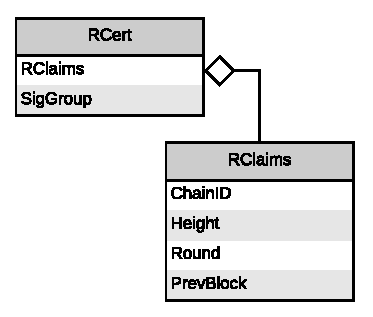
\includegraphics[scale=0.5]{figures/RCert_Object.pdf}
    \caption{RCert Object}
\end{figure}


RCert is an abbreviation of the name Round Certificate.
An RCert object wraps an RClaims object and contains a signature of the
canonical encoding of the RClaims object.
The purpose of the Round Certificate object is to allow compact proof
of consensus for a given height and round.

In order for a Round Certificate signature to be treated as valid, the
signature must be a valid group signature under the GroupKey of the
corresponding validator set for the height specified in the Round
Certificate’s RClaims object.
In round one of a given height this is the SigGroup of the BClaims
object from the block header.
This is the same requirement of a BlockHeader signature.
Thus, the round one RCert is a proof of the previous block’s hash.
In any higher round of a given height the SigGroup must be of the
RClaims object of the RCert.

The existence of a validly signed RCert implies that at least threshold
validators have provided signatures.
This either proves a new block height, in round one, or it proves a new
round has begun in some height.
This signature is a compact proof of consensus for the contents of the
RClaims or the block.


\subsection{The BClaims Object}

BClaims is an abbreviation for Block Claims.
The BClaims object encodes the proposed modifications to chain state in
a compact format.
The BClaims object is embedded, either directly or through composition,
in the BlockHeader, Proposal, PreVote, PreCommit, and NextHeight
messages.
The BClaims object does not itself carry the transactions that have
been proposed for inclusion in the next block.


\subsection{The PClaims Object}

PClaims is an abbreviation for Proposal Claims.
The PClaims object couples a Round Certificate to a set of Block Claims.
The purpose of this coupling is to prove to any participants that
observe such a message that the validators have progressed to the
specified height and round with the specified previous Block Hash.
In this way, a set of malicious validators may not vote in advance of a
round that has yet not begun according to the rules of consensus.
The PClaims object is never directly transmitted over the wire.
The PClaims object is always an embedded subobject of an actual message
type.


\subsection{The Proposal Object}

\begin{figure}[H]
    \centering
    %\includegraphics[width=3.46in,height=2.42in]{media/image5.jpg}
    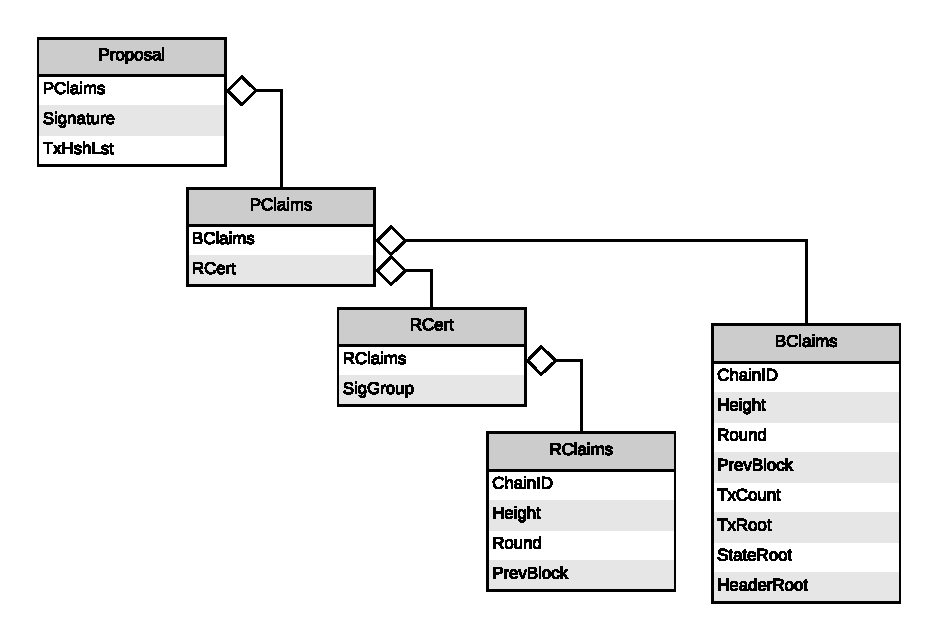
\includegraphics[scale=0.5]{figures/Proposal_Object.pdf}
    \caption{Proposal Object}
\end{figure}


The Proposal object allows a validator to propose a set of changes be
applied to the blockchain as a transactional commitment.
Only one proposal may be validly formed in a round.
This fact is an implied constraint based on two requirements of the
system.
First, there may only be one validator who is the elected proposer for
a given round.
Second, a valid proposer will only propose one value in any round.

The proposal object contains a list of all transaction hashes that
should be included in the calculation of the resulting block parameters
as described by the embedded BClaims object of a given proposal.
The acquisition of the actual transaction data is handled by an
asynchronous background operation that queries the other validators for
any unknown transaction hash.
If a validator is unable to obtain the associated data for an unknown
transaction, the validator will never vote for such a Proposal.


\subsection{The PreVote Object}

\begin{figure}[H]
    \centering
    %\includegraphics[width=3.81in,height=3.04in]{media/image12.jpg}
    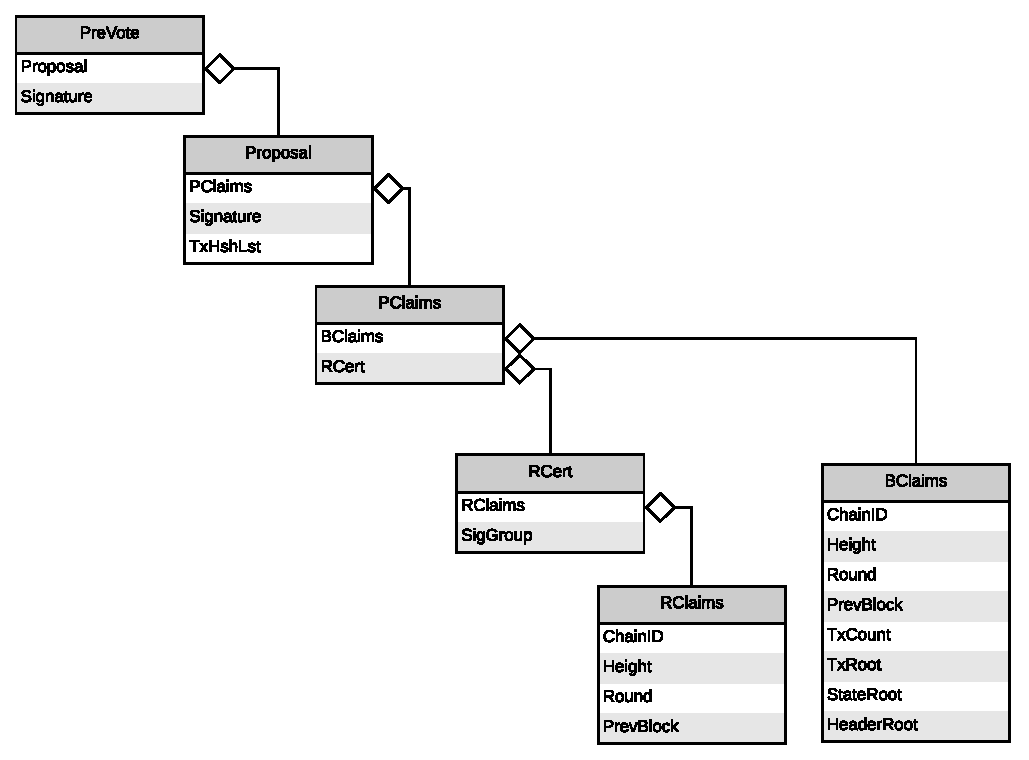
\includegraphics[scale=0.5]{figures/PreVote_Object.pdf}
    \caption{PreVote Object}
\end{figure}


The PreVote object is sent by a validator to indicate an agreement with
a proposal as the next valid state transition.
Upon receipt of a PreVote, the nested Proposal may be extracted and
applied to the state of the appropriate validator if the Proposal has
not otherwise been observed already.
A valid validator will not PreVote more than one Proposal in any round.
A valid validator will not PreVote and PreVoteNil in the same round.

\subsection{The PreVoteNil Object}

\begin{figure}[H]
    \centering
    %\includegraphics[width=2.27in,height=2.01in]{media/image2.jpg}
    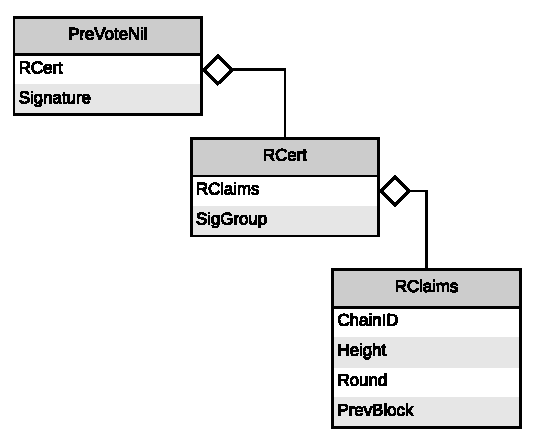
\includegraphics[scale=0.5]{figures/PreVoteNil_Object.pdf}
    \caption{PreVoteNil Object}
\end{figure}


A PreVoteNil object is sent by a validator to indicate that no valid
proposal has been observed before the ProposalTimeout or that the
validator is otherwise locked on a competing value.
A valid validator will not PreVote and PreVoteNil in the same round.
The validator does not specify a proposal in a PreVoteNil; rather, the
embedded Round Certificate acts as an identifier for a particular round
and height.
This indicator may be treated as a blanket statement for all Proposals
seen in a given round.

\subsection{The PreCommit Object}

\begin{figure}[H]
    \centering
    %\includegraphics[width=3.63in,height=2.94in]{./media/image10.jpg}
    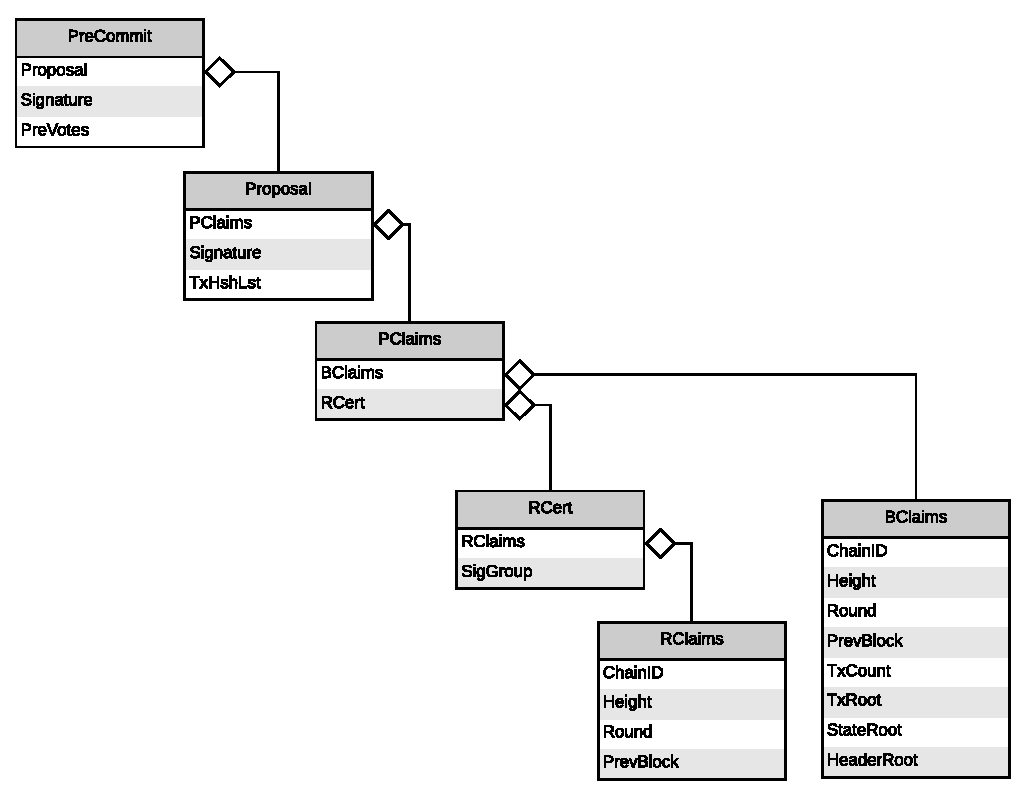
\includegraphics[scale=0.5]{figures/PreCommit_Object.pdf}
    \caption{PreCommit Object}
\end{figure}


A PreCommit object is sent by a validator to indicate that the
validator believes there is sufficient evidence to indicate that the
associated proposal will be accepted as the next state transition.
A validator may not form a valid PreCommit without having first seen at
least threshold total validators have PreVoted for the specified
Proposal in the same round.
This requirement is enforced by appending the associated signatures
from the required number of PreVotes to the PreCommit.
A valid validator may not PreCommit more than one Proposal in a round.
A valid validator will not PreCommit for a Proposal that it has also
cast a PreVoteNil for in the same round.
A validator will not PreCommit for a value that it has not cast a
PreVote for in the same round.

\subsection{The PreCommitNil Object}

\begin{figure}[H]
    \centering
    %\includegraphics[width=2.22in,height=1.75in]{media/image9.jpg}
    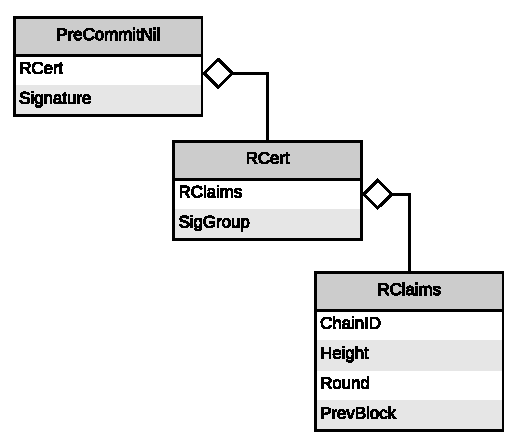
\includegraphics[scale=0.5]{figures/PreCommitNil_Object.pdf}
    \caption{PreCommitNil Object}
\end{figure}


The PreCommitNil object is sent by a validator to indicate that it has
not observed enough PreVotes to ensure a valid state transition may be
created in the current round.
A valid validator will not PreCommit and PreCommitNil\ in the same
round.


\subsection{The NextRound Object}

\begin{figure}[H]
    \centering
    %\includegraphics[width=2.35in,height=1.92in]{media/image13.jpg}
    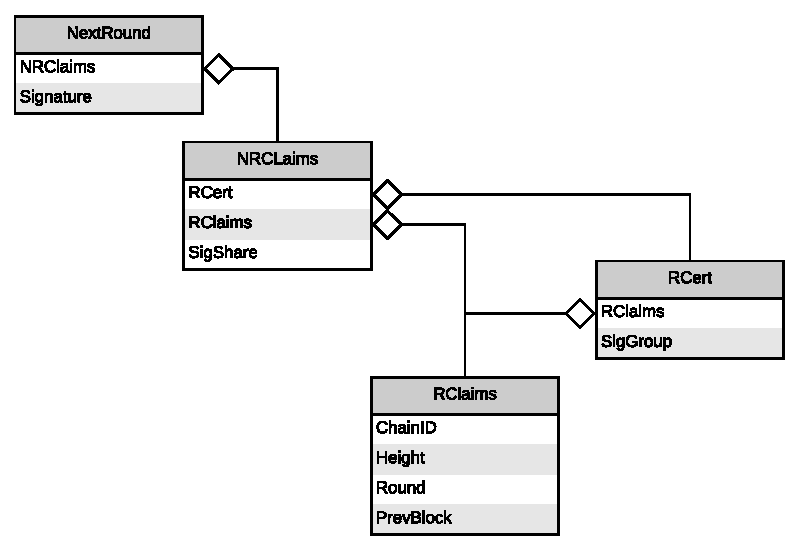
\includegraphics[scale=0.5]{figures/NextRound_Object.pdf}
    \caption{NextRound Object}
\end{figure}


The NextRound object is issued at the last phase of a round by any
validator that does not have knowledge of consensus for the next block.
This object contains two signatures.
The first signature is a secp256k1 signature of the NRClaims object.
The second signature is a BLS signature under the group share of the
validator threshold cryptosystem.
This second signature signs the RClaims object of the NRClaims object.
This RClaims object contains the same parameters as the RCert for the
current round, except the Round field has been incremented.
After observing a threshold number of NextRound messages, a new RCert
may be formed by aggregating the BLS signatures.
This provides evidence of a consensus to enter a new round.


\subsection{The NextHeight Object}

\begin{figure}[H]
    \centering
    %\includegraphics[width=3.91in,height=3.46in]{media/image8.jpg}
    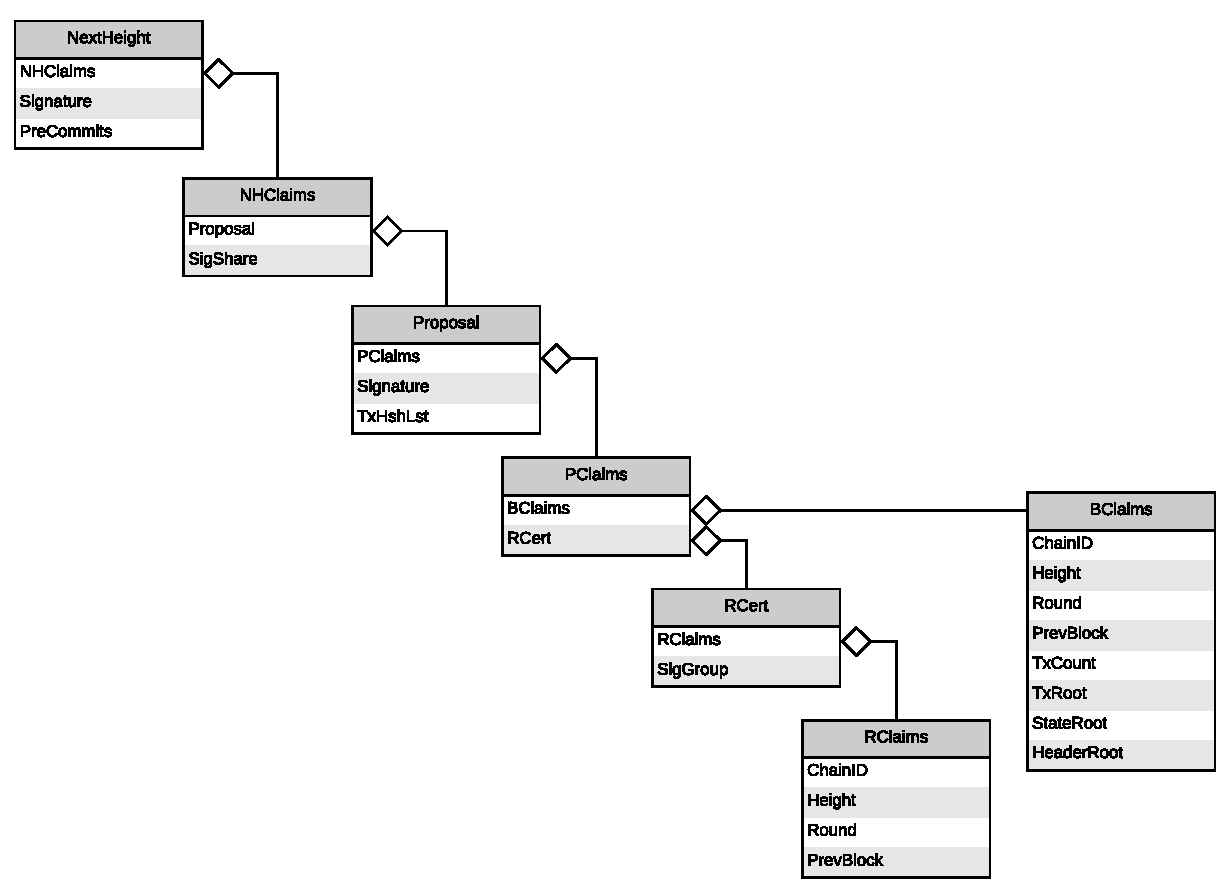
\includegraphics[scale=0.5]{figures/NextHeight_Object.pdf}
    \caption{NextHeight Object}
\end{figure}


The NextHeight object is sent by a validator that has proof of
threshold consensus in both the PreVote and PreCommit phases of
operation.
The object carries proof of this knowledge by appending the PreCommit
signatures into the message.
The NextHeight message carries two signatures.
The first signature is a signature under secp256k1 ECDSA.
The second signature is a signature under the threshold BLS key of the
validator group.
The secp256k1 key signs the canonical hash of the NHClaims objects.
The BLS signature is a signature of the BClaims object.
In this way, once a threshold number of NextHeight messages are formed,
two objects may be created.
The first object is the BlockHeader.
The second object is the round one RCert for the first round of the
next block height.
These objects are formed by creating the SigGroup object through
aggregation of the SigShare objects from threshold NextHeight objects.


\subsection{The BlockHeader Object}

\begin{figure}[H]
    \centering
    %\includegraphics[width=1.78in,height=2.33in]{media/image6.jpg}
    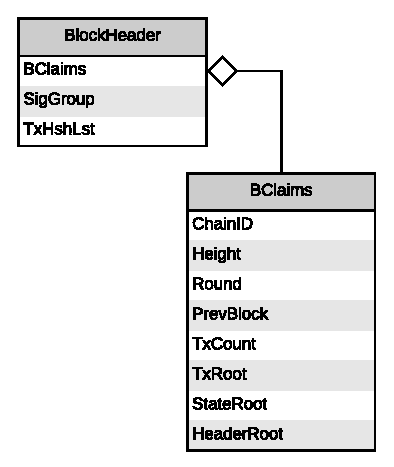
\includegraphics[scale=0.5]{figures/BlockHeader_Object.pdf}
    \caption{BlockHeader Object}
\end{figure}


A BlockHeader object may be formed following the successful completion
of a round.
This object may be formed by aggregating the BLS signatures of
threshold valid NextHeight messages.
The creation of a BlockHeader is an indication of consensus among the
validators and the BClaims described state transition.


\subsection{Validators}

A validator is an entity that performs two actions.
First, a validator must register as an entity that wishes to become a
validator using a smart contract in the Ethereum Blockchain.
This contract requires a deposit of stake at the time of this
registration.
The act of registering queues the validator up to become a new
validator in the next epoch transition if a slot is available.
The maximum number of slots the system may accommodate is 256, but the
actual system will likely be constrained to far less than this limit in
order to minimize key negotiation costs associated with the formation
of the threshold BLS signatures needed for signing BlockHeaders and
RCert objects.

Once a slot is available for the newly registered entity the second
requirement comes into force.
This requirement is that the entity is running a validating node in the
network.
This requirement is observed during the negotiation of the group key
for the validators.
Full details may be seen in the technical addendum for how this key is
negotiated and how unresponsive validators are removed.

The job of the validators is to mine new blocks into the chain and
enforce the rules of consensus.


\subsection{SnapShots}

A snapshot is performed by writing a block header into the Ethereum
blockchain.
The block header is verified as validly signed under the group key of
the validators and all fields are stored.
This value may be changed within one epoch if an invalid state
transition may be proven.
This is not possible unless greater than two thirds of the validators
collude to violate the rules of consensus.
In the event that this does occur, the guilty validators may be
identified through the Ethereum compliant secp256k1 ECDSA signatures
used to sign every consensus message type.
If no accusations are formed and proven within the epoch boundary, the
snapshot becomes canonical.


\subsection{Withdrawing From Validation}

A validator may request to be withdrawn from a role as a validator at
any time.
The validator will not be available for actual withdrawal of funds
until three epochs in the future, but the validator may not sign any
additional consensus messages at the termination of the epoch in which
the request was made.
This down time guards against malicious validators performing an attack
and then withdrawing before an accusation may be formed.


\subsection{Leader Election}

At this time the leader election algorithm is based on a simple round
robin algorithm.
This round robin algorithm does not track state across block heights.
Specifically the algorithm operates on the sum of the blockheight and
round modulo the number of validators.
A single validator is selected from a common array of validators that
every validator has available to them through the coordination of state
provided by the Ethereum blockchain.


\subsection{Virtual Votes}

The concept of a virtual vote is integral to the security of the
MadNetwork consensus algorithm.
We define a virtual vote as a vote that has been cast based on the
indirect observation of cryptographically-secure evidence.
Although the message passing protocol of the consensus algorithm may
seem overly verbose on first inspection, there is good reason.

Due to the fact that all message objects that allow the protocol to
advance in height are objects that directly embed the Proposal they
reference, and this Proposal must be cryptographically-signed, any
party who observes a PreVote, PreCommit, or NextHeight message may
extract the underlying Proposal and apply this Proposal against the
state of the validator that formed the Proposal.
The result of this operation may be one of three possible outcomes.

In the first case, the Proposal may be otherwise already known, and no
action outside the normal tracking of messages is necessary.

In the second case, the local node may not have otherwise observed any
valid Proposal from the validator that cast the Proposal.
If this is the case, the message may be applied to the validator that
formed the Proposal and the PreVote, PreCommit, or NextHeight message
may be attributed to the validator that formed the actual message.

In the third case, the Proposal may be in conflict with an already
known proposal from the associated validator for the same height and
round.
The handling of this case forms the basis for one of the most important
security assumptions of the system: no conflicting PreVotes,
PreCommits, or Proposals may be stored in the state space of a single
validator in any round such that these conflicting votes may be counted
toward consensus.

If the Proposal is in conflict, the Proposal will be discarded.
In addition to discarding the Proposal, for the message types of
PreVote and PreCommit, the validator that signed the PreVote or
PreCommit will have a virtual PreVoteNil or PreCommitNil tracked for
the purposes of consensus.
This virtual Nil vote is a placeholder to indicate that the validator
that signed the PreVote or PreCommit is not capable of voting in
agreement with the local node.
If the message that contained the Proposal is a NextHeight message, the
NextHeight is followed if the local node may validate the Proposal and
has not otherwise already performed a NextHeight operation for a
conflicting value in the same height.
If the local node has previously performed a NextHeight operation that
is in conflict, this node must follow the NextHeight it has already
locked.
This should never be possible with less than two thirds malicious
validators, but this situation may be mitigated by performing
accusations against the malicious parties in the Ethereum smart
contract system.
Since all consensus messages are signed in Ethereum compliant ECDSA,
the proof of a double proposal or a proof of signature for an
out-of-turn/invalid proposal is guaranteed to be possible.
Thus, the system will halt for a time but may re-enter consensus in the
next block by forcing the assumed value of an empty block for the
height at which the accusation was formed.

These operations are necessary because the consensus protocol requires
a threshold number of votes before progress may be made through the
steps of the protocol.
Simply discarding these messages with no additional action would cause
the protocol to halt.
Tracking these messages would add many additional layers of complexity
to the protocol.
Thus we have selected to take the course of simplification.

In summary, the tracking of virtual votes performs three functions.
First, this logic prevents the system from ever allowing two
conflicting Proposal messages to ever be stored in the database of a
single node.
Second, because this operation is performed for all PreVote and
PreCommit  message types, this prevents any conflicting votes from ever
influencing the counting of local votes that contribute to the addition
of blocks.
Third, because a virtual Nil vote may be assigned in the presence of a
conflicting vote, the algorithm may be prevented from halting due to
missing votes.


\subsection{Protocol States}

The consensus algorithm has been divided into discrete states.
The current state of the system is determined by loading all known
messages sent by the local node as well as secondary information about
the block height, round number, and authorized validators.
This operation is performed once for each iteration of the consensus
algorithm and this data is loaded directly from the database under a
protected view.
An explanation of the states and the conditions that determine a local
node’s current state will be covered shortly.

The general flow of the algorithm is to attempt consensus for a fixed
number of times at each block height.
In each block height there may be many attempts and these attempts are
named rounds.
If the maximum number of rounds is reached without consensus, the
system defaults to mining an empty block to ensure forward progress.
The flow of each round is as follows.

Each round starts with a Proposal phase where one validator forms a
proposal for the next block.
This message is transmitted to all peers and each peer gossips the
message to all other peers.
This is a flood event that is designed to prevent split view attacks.
This gossip halts at any node that has already gossiped the same
message.
This phase ends at the termination of a timeout.
At the termination of the Proposal phase each validator will PreVote or
PreVoteNil.
This is the PreVote phase that may optimistically end before a timeout
only if a threshold consensus is reached.
Otherwise, the system will force a timeout wait before entering the
next phase.
In all cases no forward progress can be made without at least threshold
votes having been observed.
The next phase is the PreCommit phase in which a validator may either
PreCommit or PreCommitNil.
This phase is also constrained by optimistic threshold progress the
same as the PreVote phase.
Lastly is the commitment phase in which round consensus is determined.
In this phase a validator may vote for a new round through a NextRound
message or a new block through a NextHeight message.
The full details are covered shortly.

The sections below will not explicitly discuss the process of gossip
since it may be treated as independent of the core operation of the
consensus algorithm for this portion of the analysis.

The approach taken to defining the consensus algorithm is far more
verbose than many approaches normally taken.
The justification for this verbosity is that although many papers
describe what is claimed to be a convergent system, this is often not
the case.
Rather than leave a possible transition as not fully defined, we have
chosen to fully expand the branch logic in the following discussion.
We were able to fully cover the truth table of possible optionality by
limiting the number of branch points.
The basis for the proof of validity of this algorithm follows this
section.

The main loop of the consensus algorithm is represented
in pseudocode in Alg.~\ref{alg:madnet_consensus}.
For simplicity, the algorithm waits for the timeouts to occur.
In practice, if we reach consensus before the timeout,
the algorithm proceeds to the next stage.

% The entire consensus algorithm in pseudocode
\begin{algorithm}[p]
\caption{Main loop of MadNet Consensus algorithm.}
\label{alg:madnet_consensus}
\begin{algorithmic}[1]
\Function{MainBlockLoop}{$ $}
    \For {$r = 1$; $r \le \textsc{DeadBlockRound}$; $r$++}
        \If {$r = \textsc{DeadBlockRound}$}
            \State \textsc{DeadBlockRoundProcedure}$()$
            \State \textbf{break}
        \EndIf
        \State $\textsc{nhBool} = \textsc{RegularRoundProcedure}()$
        \If {\textsc{nhBool}}
            \State \textbf{break}
            \Comment{Proceed to the next block height}
        \EndIf
    \EndFor
    \State \Return
\EndFunction
\end{algorithmic}
\end{algorithm}

\begin{algorithm}[p]
\caption{DeadBlockRound procedure}
\label{alg:dbr_proc}
\begin{algorithmic}[1]
\Function{DeadBlockRoundProcedure}{$ $}
    \State $\textsc{PreVote}(\textsc{EmptyBlock})$
    \State Wait until $\textsc{EmptyBlockPreVotes}\ge\textsc{Threshold}$
    \State $\textsc{PreCommit}(\textsc{EmptyBlock})$
    \State Wait until $\textsc{EmptyBlockPreCommits}\ge\textsc{Threshold}$
    \State $\textsc{NextHeight}(\textsc{EmptyBlock})$
    \State \Return
\EndFunction
\end{algorithmic}
\end{algorithm}

\begin{algorithm}[p]
\caption{Regular Round procedure}
\label{alg:rr_proc}
\begin{algorithmic}[1]
\Function{RegularRoundProcedure}{$ $}
    \State \textsc{doPendingProposalStep}$()$
    \State Wait for \textsc{ProposalTimeout}
    \State $\textsc{CurProp}, \textsc{LocalPreVote}
        = \textsc{doPendingPreVoteStep}()$
    \State Wait for \textsc{PreVoteTimeout}
    \State \textsc{doPendingPreCommitStep}(\textsc{CurProp},
        \textsc{LocalPreVote})
    \State Wait for \textsc{PreCommitTimeout}
    \State $\textsc{nhBool} = \textsc{doPendingNextStep}(\textsc{CurProp})$
    \State \Return \textsc{nhBool}
\EndFunction
\end{algorithmic}
\end{algorithm}

\begin{algorithm}[p]
\caption{Proposal procedure}
\label{alg:proposal_proc}
\begin{algorithmic}[1]
\Function{doPendingProposalStep}{$ $}
    \If {\textsc{IsProposer}$()$}
        \If {$!\textsc{LockedValueCurrent}()
                \ \land\  !\textsc{ValidValueCurrent}()$}
            \State $\textsc{NewProposal} = \textsc{MakeNewProposal}()$
            \State $\textsc{Propose}(\textsc{NewProposal})$
            \State $\textsc{ValidValue} = \textsc{NewProposal}$
        \ElsIf {$!\textsc{LockedValueCurrent}()
                \land \textsc{ValidValueCurrent}()$}
            \State $\textsc{Propose}(\textsc{ValidValue})$
        \Else
            \State $\textsc{Propose}(\textsc{LockedValue})$
        \EndIf
    \EndIf
    \State \Return
\EndFunction
\end{algorithmic}
\end{algorithm}

\begin{algorithm}[p]
\caption{PreVote procedure}
\label{alg:prevote_proc}
\begin{algorithmic}[1]
\Function{doPendingPreVoteStep}{$ $}
    \State $\textsc{CurProp} = \textsc{GetCurrentProposal}()$
    \State $\textsc{LocalPreVote} = \textsc{Nil}$
    \If {$\textsc{CurProp} \ne \textsc{Nil}$}
        \If {$!\textsc{LockedValueCurrent}()
                \ \land\  !\textsc{ValidValueCurrent}()$}
            \If {$\textsc{CurProp}.\textsc{IsValid}()$}
                \State $\textsc{PreVote}(\textsc{CurProp})$
                \State $\textsc{ValidValue} = \textsc{CurProp}$
                \State $\textsc{LocalPreVote} = \textsc{CurProp}$
            \Else
                \State $\textsc{PreVote}(\textsc{Nil})$
            \EndIf
        \ElsIf {$!\textsc{LockedValueCurrent}()
                \land \textsc{ValidValueCurrent}()$}
            \If {$\textsc{CurProp} = \textsc{ValidValue}$}
                \State $\textsc{PreVote}(\textsc{ValidValue})$
                \State $\textsc{LocalPreVote} = \textsc{CurProp}$
            \Else
                \State $\textsc{PreVote}(\textsc{Nil})$
            \EndIf
        \Else
            \If {$\textsc{CurProp} = \textsc{LockedValue}$}
                \State $\textsc{PreVote}(\textsc{LockedValue})$
                \State $\textsc{LocalPreVote} = \textsc{CurProp}$
            \Else
                \State $\textsc{PreVote}(\textsc{Nil})$
            \EndIf
        \EndIf
    \Else
        \State $\textsc{PreVote}(\textsc{Nil})$
        \Comment{No current proposal}
    \EndIf
    \State \Return \textsc{CurProp}, \textsc{LocalPreVote}
\EndFunction
\end{algorithmic}
\end{algorithm}

\begin{algorithm}[p]
\caption{PreCommit procedure}
\label{alg:precommit_proc}
\begin{algorithmic}[1]
\Function{doPendingPreCommitStep}{\textsc{CurProp}, \textsc{LocalPreVote}}
    \State $\textsc{NumPreVotes}
        = \textsc{GetCurrentPreVotes}(\textsc{CurProp})$
    \If {$\textsc{NumPreVotes} \ge \textsc{Threshold}$}
        \State $\textsc{ValidValue} = \textsc{CurProp}$
        \If {$\textsc{CurProp} = \textsc{LocalPreVote}$}
            \State $\textsc{PreCommit}(\textsc{CurProp})$
            \State $\textsc{LockedValue} = \textsc{CurProp}$
            \State \Return
        \Else
            \State $\textsc{ValidValue} = \textsc{CurProp}$
        \EndIf
    \EndIf
    \State $\textsc{PreCommit}(\textsc{Nil})$
    \State \Return
\EndFunction
\end{algorithmic}
\end{algorithm}

\begin{algorithm}[p]
\caption{NextStep procedure}
\label{alg:nextstep_proc}
\begin{algorithmic}[1]
\Function{doPendingNextStep}{$\textsc{CurProp}$}
    \State $\textsc{nhBool} = \textsc{False}$
    \State $\textsc{NumPreCommits}
        = \textsc{GetCurrentPreCommits}(\textsc{CurProp})$
    \If {$\textsc{NumPreCommits} \ge \textsc{Threshold}$}
        \State $\textsc{NextHeight}(\textsc{CurProp})$
        \State $\textsc{nhBool} = \textsc{True}$
    \Else
        \State \textsc{NextRound}$()$
    \EndIf
    \State \Return \textsc{nhBool}
\EndFunction
\end{algorithmic}
\end{algorithm}


\afterpage{\clearpage}


\subsubsection{PendingProposal}

Possible Next States:

\begin{itemize}
    \item RoundJump
    \item HeightJump
    \item FormNextHeight
    \item ProposalStep
    \item PendingProposal
    \item PendingPreVote
\end{itemize}

A valid node that has entered this state has not cast a Proposal,
PreVote, PreVoteNil, PreCommit, PreCommitNil, or NextRound vote for the
current round.
The ProposalTimeout, the PreVoteTimeout, and the
PreCommitTimeout have not expired for this round.
The node has not seen a valid NextHeight message for the current height.
The node has not seen a message for a higher round in the same height.
The node has not seen a valid message for a higher BlockHeight.

If the local node is the proposer for the current round and neither
ValidValue or LockedValue are from the same height as the current
round, the validator will form a new proposal.
The validator will write this Proposal to the database and store this
Proposal as ValidValue in the database as well.

If the local node is the proposer for the current round and ValidValue
is from the current height, but LockedValue is not from the current
height, the validator will propose the value defined by ValidValue and
will set ValidValue equal to the constructed Proposal.
The validator may then return.

If the local node is the proposer for the current round and LockedValue
is from the current height, but ValidValue is not from the current
height, the validator will propose the value defined by LockedValue and
will set ValidValue equal to the constructed Proposal.
The validator may then return.

All logic below this point is guarded by the condition that ValidValue
and LockedValue are of the same blockheight as the current round.

If the local node is the proposer for the current round and the round
number of ValidValue is greater than the round number for LockedValue,
then ValidValue will be proposed and the validator will set ValidValue
equal to the constructed Proposal.
The validator may then return.

If the local node is the proposer for the current round and the round
number for LockedValue is greater than the round number for ValidValue,
then the value defined by LockedValue will be proposed and the
validator will set ValidValue equal to the constructed Proposal.
The validator may then return.

If the local node is the proposer for the current round and both
LockedValue and ValidValue are from the same round number, then the
value defined by LockedValue will be proposed and the validator will
set ValidValue equal to the constructed Proposal.
The validator may then return.

If the local node is not the proposer for the current round, the node
may immediately return without performing any work.

In order to give the reader insight as to what the structure of the
previous statements look like in the actual implementation, the
following code is provided from the source code of the MadNetwork
repository; see Listing~\ref{list:dPP}.
The intent of including this example code is to allow the reader to
understand how the conditional structures have been implemented.
We have gone to great lengths to structure the code of the consensus
algorithm as fully covering truth tables where possible to increase
readability.

\lstset{language=Go,
    keywordstyle=\color{blue}\bfseries,
    commentstyle=\color{green!50!black},
    stringstyle=\ttfamily\color{red!50!brown},
    showstringspaces=false,
    frame=single
}
{
\small
\lstinputlisting[label=list:dPP,float,language=Go,caption=Pending Proposal Step]{code/doPendingProposalStep.go}
}



\subsubsection{ProposalStep}

Possible Next States:

\begin{itemize}
    \item RoundJump
    \item HeightJump
    \item FormNextHeight
    \item ProposalStep
    \item PendingPreVote
\end{itemize}

A valid node that has entered this state is a designated proposer for
the current round who has cast a Proposal but has not cast a PreVote,
PreVoteNil, PreCommit, PreCommitNil, NextRound, or NextHeight vote for
the current round.
The ProposalTimeout, the PreVoteTimeout, and the PreCommitTimeout have
not expired for this round.
Further, the node has not seen a valid NextHeight message for the
current height.

The node may immediately return without performing any work.

This state is a logically empty state that is intended to guard against
a double proposal.


\subsubsection{PendingPreVote}

Possible Next States:

\begin{itemize}
    \item RoundJump
    \item HeightJump
    \item FormNextHeight
    \item PreVoteStep
    \item PreVoteNilStep
\end{itemize}

A valid node that has entered this state has not cast a PreVote,
PreVoteNil, PreCommit, PreCommitNil, NextRound, or NextHeight vote for
the current round, and the ProposalTimeout has expired.
The PreVoteTimeout and the PreCommitTimeout have not expired for this
round.
Further, the node has not seen a valid NextHeight message for the
current height.

If the local node is not a validator for the current round, the node
may return without performing any additional work.
The following logic is guarded by this conditional.

If a validator has received a Proposal that it has been able to verify
as valid, then that proposal shall be called the PendingProposal for
the purpose of this section.
If the validator has not received a Proposal that it was able to verify
as valid, then the PendingProposal shall be considered equal to the
value Nil for the purpose of this section.

If the PendingProsposal is Nil, the validator will store a PreVoteNil
in the local database and return.

If the PendingProsposal is not equal to Nil, the PendingProposal must
be checked for validity with respect to the state transition.
All logic below this point is guarded by the condition that the
PendingProposal is not Nil.

If the PendingProposal may be verified as invalid, the validator may
write a PreVoteNil to the database and return.

If the PendingProposal may be verified as valid, then the LockedValue
and ValidValue must be checked for equivalence and recency.
All logic below this point is guarded by the conditions that the
PendingProposal is not Nil and has been verified as valid with respect
to the state transition of the system.

If neither the ValidValue or LockedValue is from the current height,
the validator may write a PreVote for the PendingProposal to the
database and return.

If ValidValue is from the current height, but LockedValue is not from
the current height, and the PendingProposal and the ValidValue are for
the same BClaims object, then the validator will write a PreVote for
the PendingProposal to the database and return.

If ValidValue is from the current height, but LockedValue is not from
the current height, and the PendingProposal and the ValidValue are not
for the same BClaims object, then the validator will write a PreVoteNil
to the database for the current round and return.

If LockedValue is from the current height, but ValidValue is not from
the current height, and the PendingProposal and the LockedValue are for
the same BClaims object, then the validator will write a PreVote for
the PendingProposal to the database and return.

If LockedValue is from the current height, but ValidValue is not from
the current height, and the Pending proposal and the LockedValue are
not for the same BClaims object, then the validator will write a
PreVoteNil to the database for the current round and return.

If both the ValidValue and the LockedValue are from the current height,
then the round numbers will be compared.
All logic below this point is guarded by the condition that the
ValidValue and the LockedValue are both for the same height and that
height is equal to the height of the current round.

If the round number of the ValidValue is greater than the round number
of the LockedValue, and the PendingProposal and the ValidValue are for
the same BClaims object, then the validator will write a PreVote for
the PendingProposal to the database and return.

If the round number of the ValidValue is greater than the round number
of the LockedValue, and the Pending proposal and the ValidValue are not
for the same BClaims object, then the validator will write a PreVoteNil
to the database for the current round and return.

If the round number of the LockedValue is greater than the round number
of the ValidValue, and the PendingProposal and the LockedValue are for
the same BClaims object, then the validator will write a PreVote for
the PendingProposal to the database and return.

If the round number of the LockedValue is greater than the round number
of the ValidValue, and the Pending proposal and the LockedValue are not
for the same BClaims object, then the validator will write a PreVoteNil
to the database for the current round and return.

If the round number of the LockedValue and the ValidValue are equal,
and the PendingProposal and the LockedValue are for the same BClaims
object, then the validator will write a PreVote for the PendingProposal
to the database and return.

If the round number of the LockedValue and the ValidValue are equal,
and the Pending proposal and the LockedValue are not for the same
BClaims object, then the validator will write a PreVoteNil to the
database for the current round and return.


\subsubsection{PreVoteNilStep}

\begin{itemize}
    \item RoundJump
    \item HeightJump
    \item FormNextHeight
    \item PreVoteNilStep
    \item PendingPreCommit
    \item PreCommitNilStep
\end{itemize}

A valid node that has entered this state has cast a PreVoteNil for the
current round.
A node that has entered this state has not cast a PreVote, PreCommit,
PreCommitNil, NextRound, or NextHeight vote for the current round, and
the ProposalTimeout has expired.
The PreVoteTimeout and the PreCommitTimeout have not expired for this
round.
Further, the node has not seen a valid NextHeight message for the
current height.

If the local node is not a validator for the current round, the node
may return without performing any additional work.
The following logic is guarded by this conditional.

Upon entering this state, the node will first count the number of
PreVote and PreVoteNil messages observed for the current round.

If greater than threshold PreVotes has been seen for this round, the
node will write a PreCommitNil for the current round to the database.
The node will also write the Proposal that has greater than threshold
PreVotes to the database as ValidValue.
The node may then return.

If greater than threshold PreVoteNils has been seen for this round, the
node will write a PreCommitNil for the current round to the database
and return.

If neither the number of PreVotes or the number of PreVoteNil messages
is greater than the threshold, the node may return without performing
any additional work.


\subsubsection{PreVoteStep}

Possible Next States:

\begin{itemize}
    \item RoundJump
    \item HeightJump
    \item FormNextHeight
    \item PreVoteStep
    \item PendingPreCommit
    \item PreCommitStep
\end{itemize}

A valid node that has entered this state has cast a PreVote for the
current round.
A node that has entered this state has not cast a PreVoteNil,
PreCommit, PreCommitNil, NextRound, or NextHeight vote for the current
round, and the ProposalTimeout has expired.
The PreVoteTimeout and the PreCommitTimeout have not expired for this
round.
Further, the node has not seen a valid NextHeight message for the
current height.

If the local node is not a validator for the current round, the node
may return without performing any additional work.
The following logic is guarded by this conditional.

Upon entering this state, the node will first count the number of
PreVote and PreVoteNil messages observed for the current round.

If greater than threshold PreVotes has been seen for this round, the
node will write a PreCommit for the current round to the database.
The node will store the Proposal associated with the PreCommit to the
database as the ValidValue.
The node will store the Proposal associated with the PreCommit to the
database as the LockedValue.
The node may then return.

If greater than threshold PreVoteNils has been seen for this round, the
node will write a PreCommitNil for the current round to the database
and return.

If neither the number of PreVotes or the number of PreVoteNils is
greater than the threshold, the node may return without performing any
additional work.


\subsubsection{PendingPreCommit}
Possible Next States:

\begin{itemize}
    \item RoundJump
    \item HeightJump
    \item FormNextHeight
    \item PreCommitNilStep
    \item PreCommitStep
\end{itemize}

A valid node that has entered this state has cast either a PreVote or
a PreVoteNil for the current round.
A node that has entered this state has not cast a  PreCommit,
PreCommitNil, NextRound, or NextHeight vote for the current round.
Both the ProposalTimeout and the PreVoteTimeout have expired for this
round.
The PreCommitTimeout has not expired for this round.
Further, the node has not seen a valid NextHeight message for the
current height.

If the local node is not a validator for the current round, the node
may return without performing any additional work.
The following logic is guarded by this conditional.

Upon entering this state, the node will first count the number of
PreVote and PreVoteNil messages observed for the current round.

If the local node has cast a PreVote in the current round and the
number of PreVotes is greater than the threshold, the node will write a
PreCommit for the current round to the database.
The node will also store the Proposal associated with the PreCommit to
the database as the ValidValue.
The node will also store the Proposal associated with the PreCommit to
the database as the LockedValue.
The node may then return.

If the local node has cast a PreVoteNil in the current round and the
number of PreVotes is greater than the threshold, the node will write a
PreCommitNil for the current round to the database.
The node will also store the Proposal associated with the PreVotes to
the database as the ValidValue.
The node may then return.

If the local node has cast a PreVote in the current round and the
number of PreVotes observed in the current round is less than the
threshold and the sum of the number of PreVotes and PreVoteNils in the
current round is greater than the threshold, the node will write a
PreCommitNil to the database.
The node may then return.

If the local node has cast a PreVoteNil in the current round and the
number of PreVotes observed in the current round is less than the
threshold and the sum of the number of PreVotes and PreVoteNils in the
current round is greater than the threshold, the node will write a
PreCommitNil to the database and return.

If none of the above conditions hold, the node may return without
performing any additional work.


\subsubsection{PreCommitNilStep}

Possible Next States:

\begin{itemize}
    \item RoundJump
    \item HeightJump
    \item FormNextHeight
    \item PreCommitNilStep
    \item NextRound
    \item NextHeight
\end{itemize}

A valid node that has entered this state has cast a PreCommitNil for
the current round.
A node that has entered this state has not cast a PreCommit, NextRound,
or NextHeight vote for the current round.
The ProposalTimeout has expired for this round.
The PreVoteTimeout may have expired for this round.
The PreCommitTimeout has not expired for this round.
Further, the node has not seen a valid NextHeight message for the
current height.

If the local node is not a validator for the current round, the node
may return without performing any additional work.
The following logic is guarded by this conditional.

Upon entering this state, the node will first count the number of
PreCommit and PreCommitNil messages observed for the current round.

If the number of PreCommits is greater than the threshold and the node
is capable of validating the Proposal associated with the PreCommits as
performing a valid state transition, then the local node may write a
NextHeight message to the database for the current round and return.

If the number of PreCommitNils is greater than the threshold and the
number of PreCommits is greater than the zero, and the node is capable
of validating that the Proposal associated with the PreCommit results
in a valid state transition, the node will store the Proposal
associated with the PreCommit to the database as the ValidValue.
The node will also write to the database a NextRound for the current
round and return.

If the number of PreCommitNils is greater than the threshold and the
number of PreCommits is equal to zero the node will write to the
database a NextRound for the current round and return.

If none of the above conditions hold, the node may return without
performing any additional work.


\subsubsection{PreCommitStep}

Possible Next States:

\begin{itemize}
    \item RoundJump
    \item HeightJump
    \item FormNextHeight
    \item PreCommitStep
    \item NextRound
    \item NextHeight
\end{itemize}

A valid node that has entered this state has cast a PreVote and
PreCommit for the current round.
A node that has entered this state has not cast a PreCommitNil,
NextRound, or NextHeight vote for the current round.
The ProposalTimeout has expired for this round and the PreVoteTimeout
may have expired for this round.
The PreCommitTimeout has not expired for this round.
Further, the node has not seen a valid NextHeight message for the
current height.

If the local node is not a validator for the current round, the node
may return without performing any additional work.
The following logic is guarded by this conditional.

Upon entering this state, the node will first count the number of
PreCommit and PreCommitNil messages observed for the current round.

If the number of PreCommits is greater than threshold, the node will
write a NextHeight message to the database and return.

If the number of PreCommitNils is greater than threshold, the node will
write a Next\-Round message to the database and return.

If neither the number of PreCommits or the number of PreCommitNils is
greater than the threshold, the node will return without performing any
additional work.


\subsubsection{PendingNext}

Possible Next States:

\begin{itemize}
    \item RoundJump
    \item HeightJump
    \item FormNextHeight
    \item PendingNext
    \item NextRound
    \item NextHeight
\end{itemize}

A valid node that has entered this state has cast a PreCommit or a
PreCommitNil for the current round.
A node that has entered this state has not cast a NextRound or
NextHeight vote for the current round.
The ProposalTimeout, the PreVoteTimeout, and the PreCommitTimeout have
expired for this round.
Further, the node has not seen a valid NextHeight message for the
current height.

If the local node is not a validator for the current round, the node
may return without performing any additional work.
The following logic is guarded by this conditional.

Upon entering this state, the node will first count the number of
PreCommit and PreCommitNil messages observed for the current round.

If the local node has cast a PreCommit in this round, and the number of
PreCommits is greater than threshold, the node will write a NextHeight
message to the database and return.

If the local node has cast a PreCommitNil in this round, the number of
PreCommits is greater than threshold, and the local node is capable of
validating the Proposal associated with the PreCommits, the node will
write a NextHeight message to the database and return.

If the local node has cast a PreCommitNil in this round, the number of
PreCommits is greater than threshold, and the local node is not capable
of validating the Proposal associated with the PreCommits, the node will
return without doing any further work.

If the number of PreCommits is less than threshold, but the sum of the
PreCommits and the PreCommitNils is greater than the threshold, the
local node will write a NextRound message to the database and return.


\subsubsection{NextRoundStep}

Possible Next States:

\begin{itemize}
    \item RoundJump
    \item HeightJump
    \item FormNextHeight
    \item PendingNext
    \item NextRound
    \item NextHeight
    \item PendingProposal
\end{itemize}

A valid node that has entered this state has cast a PreCommit or a
PreCommitNil for the current round.
A node that has entered this state has not cast a NextHeight vote for
the current round.
The ProposalTimeout has expired for this round.
The PreVoteTimeout may have expired for this round.
The PreCommitTimeout may have expired for this round.
Further, the node has not seen a valid NextHeight message for the
current height.

If the local node is not a validator for the current round, the node
may return without performing any additional work.
The following logic is guarded by this conditional.

Upon entering this state, the node will first count the number of
PreCommit and PreCommitNil messages observed for the current round.
Upon entering this state, the node will also count the number of
NextRound messages observed for the current round.

If the local node has cast a PreCommit in this round, and the number of
PreCommits is greater than threshold, the node will write a NextRound
message to the database and return.

If the local node has cast a PreCommitNil in this round, the number of
PreCommits is greater than threshold, and the local node is capable of
validating the Proposal associated with the PreCommits the node will
write a NextRound message to the database and return.

If the local node has cast a PreCommitNil in this round, the number of
PreCommits is greater than threshold, and the local node is not capable
of validating the Proposal associated with the PreCommits the node will
return without doing any further work.

If the local node has not seen greater than threshold PreCommits, and
has not seen greater than threshold NextRound messages, the node may
return without doing any further work.

If the local node has not seen greater than threshold PreCommits, and
has seen greater than threshold NextRound messages, the node will write
to the database a new RoundCert object and return.


\subsubsection{NextHeightStep}

Possible Next States:

\begin{itemize}
    \item HeightJump
    \item NextHeight
    \item PendingProposal
\end{itemize}

A valid node that has entered this state has cast a NextHeight message
for the current height.

There are no other guarantees about the state of this node.

If the local node is not a validator for the current round, the node
may return without performing any additional work.
The following logic is guarded by this conditional.

Upon entering this state, the node will first count the number of
NextHeight messages observed for the current height.

If the number of NextHeight messages is greater than threshold, the
validator will form a new BlockHeader and write it to the database.

If the number of NextHeight messages is not greater than threshold, the
validator may return without performing any additional work.


\subsubsection{RoundJump}

Possible Next States:

\begin{itemize}
    \item HeightJump
    \item FormNextHeight
    \item PendingProposal
\end{itemize}

A valid node that has entered this state has observed a valid Round
Certificate with a higher round number in the same height as the
current round.
Further, the node has not seen a valid NextHeight message for the
current height.

The node will write the new RCert to the database in the location of
the local nodes MostRecentRoundCert and return.


\subsubsection{HeightJump}

Possible Next States:

\begin{itemize}
    \item RoundJump
    \item HeightJump
    \item FormNextHeight
    \item PendingProposal
\end{itemize}

A valid node that has entered this state has seen a validly signed
BlockHeader or Round Certificate for a height that is greater than the
height of the current round.

If the height of the BlockHeader or Round Certificate is equal to one
greater than the current round of the validator, and the PrevBlock
value of the Round Certificate or BlockHeader is equal to the the
expected blockhash from the current ValidValue, LockedValue, or the
most recent PreVote that the local node cast, store the BlockHeader and
return.

If the height of the BlockHeader or Round Certificate is equal to one
greater than the current round of the validator, and the PrevBlock
value of the Round Certificate or BlockHeader is NOT equal to the the
expected blockhash from the current ValidValue, LockedValue, or the
most recent PreVote that the local node cast, perform no additional
work and return.

If the height is greater than one more than the height of the current
round, return without performing any additional work.

Note: This logic was chosen to allow the synchronization protocol to
perform the work necessary to bring the node up to the correct height.


\subsubsection{FormNextHeight}

Possible Next States:

\begin{itemize}
    \item RoundJump
    \item HeightJump
    \item FormNextHeight
    \item NextHeight
\end{itemize}

A valid node that has entered this state has seen a valid NextHeight
message for the current height.

There are no other guarantees about the state of this node.

Form a NextHeight message.
Write the message to the database and return.


\subsection{Mining Rewards}

Mining rewards take two forms at this time.
First, a validator is rewarded for cleaning up stale DataStore objects
from the chain.
Second, a validator is paid a base reward in tokens for performing the
function of being a validator.
These rewards are distributed in the block snapshotting process and are
minted into the Ethereum blockchain.
These rewards are not available for transfer or use until after at
least one additional snapshot has been written to the Ethereum
blockchain.


\subsection{Slashing}

In order to ensure the miners are honest, there is not only the
possibility of mining rewards for following the protocol but also
the threat of punishment for misbehavior.
There will be two types of fines: major fine and minor fine.
A major fine is any fine that can be cryptographically-verifiable
malicious action.
These include submitting incorrect shares or group public keys during
the DKG process.
While mining blocks, double-signing at a given block height is
also malicious.
A major fine should reduce a validator's stake to the point where he
is unable to proceed with the DKG process.
A minor fine may occur during the DKG process when a validator fails
to submit the appropriate information.
Because it is possible this was the result of technical failure and
not malicious intent, we believe this should not be as large of a fine.
Even so, validators are a critical part of the process and are expected
to be resilient against technical failures.


\subsection{Consensus Proofs}

We now turn our attention to proving the safety of our consensus
algorithm.
This will follow from a number of lemmas.


\subsubsection{Safety}

The arguments of safety and fault tolerance for the system are natural
extensions of the proofs for the ancestral origin of both the consensus
mechanism and its parent.
These algorithms are, respectively, DLS and Tendermint.

We build our model in the case of Partial Synchrony.
Specifically, we assume that all messages that are sent must be
eventually received.
The sending of this message may be accomplished in a single attempt, or
it may be accomplished through multiple retransmissions.
In either case the message will be received and handled.
Messages may arrive in any order and may arrive more than once.
We aim for the following properties:

\begin{itemize}
	\item All valid nodes decide on the same valid output value.
	\item All valid nodes eventually decide on some valid output value.
	\item A value is defined as valid if it satisfies a predefined
    predicate \textit{isValid()}.
\end{itemize}

Our algorithm operates in the model of total group order equal to $3f+1$
with a threshold of $2f+1$ in order to ensure progress.
Thus, we may tolerate up to $f$ faults.
Our system can tolerate strictly less than one-third Byzantine failures.
We built our system to ensure safety even in the presence of greater
than one-third total failures as long as we limit Byzantine failures to
strictly less than one-third.
This design principle does come with the necessary sacrifice of
liveliness under the conditions that failures exceed the allowable
threshold.

This section will be written entirely in the context of consensus and
will not speak about this information in terms of transactions.
We will speak about the system in terms of blocks and values, where a
block represents an append-only operation onto a shared distributed log
and a value will be a portion of the contents of the object appended to
this log.
For the purpose of this discussion, we may assume all other fields
within this object are deterministically created based on application
state and the proposed value itself.


\subsubsection{Rules}

If you PreCommit a Proposal in any round at any height, you will set
LockedValue equal to the Proposal that you PreCommitVoted and you will
not unset this value at the same block height in any round before
signing the NextRound message that would lead to the DeadBlockRound.

After signing the NextRound message that would lead to the
DeadBlockRound for a given block height, you must unset LockedValue and
ValidValue.

After signing the NextRound message that would lead to the
DeadBlockRound for a given block height, you must ignore any NextHeight
message from any previous round.


\subsubsection{Proof of Safety}

The proof of safety relies on this observation from
Lemma~\ref{lem:threshold_subsets}: two subsets with at least
a threshold number of validators in each subset will share at least one
honest validator.

\begin{lem}
\label{lem:threshold_subsets}
Let $f$ be the number of malicious validators.
Given any two subsets with at least $2f+1$ validators in a system
containing $3f+1$ validators, those two subsets share at least $f+1$ validators.
Thus, these two subsets share at least one honest validator.
\end{lem}

\begin{proof}
Let $A$ and $B$ be two subsets with at least $2f+1$ validators
chosen from $N = 3f+1$ validators.
From De Morgan’s laws, we know

\begin{equation*}
    A \cap B = (A^{c} \cup B^{c})^{c}.
\end{equation*}

\noindent
Here, $A^{c}$ denotes the complement of $A$ (that is, the elements of the
system not in A).
In what follows, $\abs{A}$ denotes the number of elements in $A$.
Thus, we have

\begin{align*}
    \abs{A\cap B} &= \abs{(A^{c} \cup B^{c})^{c}} \\
        &= N - \abs{A^{c} \cup B^{c}} \\
        &\ge N - \parens{\abs{A^{c}} + \abs{B^{c}}} \\
        &\ge N - 2f \\
        &= f + 1.
\end{align*}

\noindent
Their intersection shares at least $f+1$ validators and there are $f$
malicious validators, so we see that $A$ and $B$ share at least one honest
validator.
\end{proof}

This lemma ensures that honest participants will always agree when
PreCommitting a proposal or submitting a NextHeight message in a given
round, as the next two lemmas show.

\begin{lem}
\label{lem:2_honest_precommit}
In any round, any 2 honest participants who PreCommit a proposal will PreCommit
the same proposal.
\end{lem}

\begin{proof}
Suppose two honest participants PreCommit proposals $P_{1}$ and $P_{2}$.
To PreCommit a proposal, they both must have knowledge of at least $2f+1$
PreVote messages from participants.
There corresponds subsets $S_{1}$ and $S_{2}$, where $S_{1}$ contains
the participants who submitted prevotes for $P_{1}$ and $S_{2}$ contains
the participants who submitted PreVotes for $P_{2}$.
By Lemma~\ref{lem:threshold_subsets},
$S_{1}$ and $S_{2}$ share at least one honest participant.
An honest participant will only PreVote for one value in a round, so the
proposals $P_{1}$ and $P_{2}$ must agree.
\end{proof}

\begin{lem}
\label{lem:2_honest_nextheight}
In any round, any 2 honest participants who submit a NextHeight message
will submit a NextHeight message for the same proposal.
\end{lem}

\begin{proof}
Mutatis mutandis, the proof is the same as that of
Lemma~\ref{lem:2_honest_precommit}.
\end{proof}

We are now able to show the multiple distinct NextHeight messages from honest
participants are not able to occur before the DeadBlockRound.
This is a stronger result than Lemma~\ref{lem:2_honest_nextheight}
and follows from the fact that a
threshold number of LockedValues must occur before submitting a NextHeight
message.

\begin{lem}
\label{lem:2_distinct_nextheight}
In any round before the DeadBlockRound, any 2 honest participants
who submit a NextHeight message will submit a NextHeight message
for the same proposal.
\end{lem}

\begin{proof}
Suppose we have not yet reached the DeadBlockRound.
Let $P_{1}$ and $P_{2}$ be NextHeight messages from two honest participants
with corresponding signing subsets $S_{1}$ and $S_{2}$.
When $P_{1}$ is signed, all members of $S_{1}$ are supposed to set
LockedValue to the proposal corresponding to $P_{1}$ because they
PreCommitted $P_{1}$.
Similarly, all members of $S_{2}$ are supposed to set LockedValue
to the proposal corresponding to $P_{2}$ because they PreCommitted $P_{2}$.
This implies $S_{1}$ and $S_{2}$ are two subsets of participants of size
at least $2f+1$ with LockedValue set.
Once an honest participant sets his LockedValue, it is never unset before the
DeadBlockRound.
By Lemma~\ref{lem:threshold_subsets},
$S_{1}$ and $S_{2}$ have at least one honest participant in common
with his LockedValue set to one proposal.
Thus, we see that the $P_{1}$ and $P_{2}$ NextHeight messages must be
for the same proposal when they are submitted by honest participants.
\end{proof}

Lemma~\ref{lem:honest_signed_nextround}
is useful in bounding the number of honest validators who may not
proceed to the next round.

\begin{lem}
\label{lem:honest_signed_nextround}
In order for $2f+1$ validators to enter a round, at least $f+1$
honest validators must have signed a NextRound message and at most $f$
honest validators failed to sign a NextRound message.
\end{lem}

\begin{proof}
We recall an honest validator may not enter a round without a valid
RoundCertificate.
A NextRound message contains two objects.
The first object is a RoundCertificate for the current round.
The second is a RoundShare object for the next round.
A RoundCertificate contains both round number and block height as internal
fields, and in order to form a valid Round Certificate, at least $2f+1$
validators must have signed a RoundShare.
Because there are at most $f$ dishonest validators who signed for the
RoundCertificate, at least $f+1$ honest validators must have also signed the
RoundCertificate.
Thus, at most $f$ honest validators did not sign the RoundCertificate.
\end{proof}

Once validators reach the DeadBlockRound, they will not acknowledge any
NextHeight messages for any preceding round.
This ensures that dishonest validators are not able to fork the chain by
producing a block based on those NextHeight messages.

\begin{lem}
\label{lem:sign_rc_dbr}
If at least $2f+1$ participants sign the RoundCertificate to the DeadBlockRound,
then it is not possible for $2f+1$ participants to form a valid NextHeight
message for any round preceding the DeadBlockRound.
\end{lem}

\begin{proof}
Given Lemma~\ref{lem:honest_signed_nextround}
and the rule that any honest validator who has signed a
NextRound message for the DeadBlockRound will never sign or acknowledge any
NextHeight message from a previous round, at least $f+1$ honest validators must
have signed a NextRound message for the DeadBlockRound if there exists a
RoundCertificate for the DeadBlockRound.
If at least $f+1$ honest validators are in the DeadBlockRound,
at most $f$ honest validators may remain in a round preceding
the DeadBlockRound.
If at most $f$ honest validators remain in a preceding round, then the malicious
validators are unable to use the signatures of $f$ honest validators to form a
set of $2f+1$ valid NextHeight messages.
Therefore, the malicious validators may not form a block from those NextHeight
messages.
\end{proof}

With this assurance, we allow for participants to safely proceed to the
DeadBlockRound even if they previously were locked onto a NextHeight message.

\begin{lem}
\label{lem:safe_unlock_nh_dbr}
It is safe for any participant who is locked on a NextHeight message to unlock
and proceed to the DeadBlockRound upon receiving a RoundCertificate for the
DeadBlockRound.
\end{lem}

\begin{proof}
This follows from Lemma~\ref{lem:sign_rc_dbr}.
\end{proof}

The previous work allows us to show that we will converge to the EmptyBlock
when a RoundCertificate for the DeadBlockRound exists.
This ensures new blocks will be created even if no transactions are performed.

\begin{lem}
\label{lem:emptyblock_rc_dbr}
The DeadBlockRound must converge to the EmptyBlock if a RoundCertificate for
the DeadBlockRound exists.
\end{lem}

\begin{proof}
Upon entering the DeadBlockRound, every valid process will immediately PreVote
the EmptyBlock and ignore all other contradicting votes.
These contradicting votes include any PreVote for a Proposal that is not the
EmptyBlock, any NextRound message, any PreCommit that is not a PreCommit for
the EmptyBlock, and any PreVoteNil or PreCommitNil message as well.
As a result of Lemma~\ref{lem:sign_rc_dbr},
at least $f+1$ honest validators enter the DeadBlockRound.
Therefore, the honest validators who enter the DeadBlockRound will only
progress once at least $f$ other validators also PreVote in the DeadBlockRound.
Because we assume all messages are eventually received, the at most $f$ honest
validators who did not sign the NextRound Certificate for the DeadBlockRound
will eventually receive the RoundCertificate for the DeadBlockRound and PreVote
for the EmptyBlock in the DeadBlockRound.
It follows that the round eventually converges to the EmptyBlock and no other
possible block.
\end{proof}

The previous work also allows us to show we will not converge to more
than one valid block at a given block height.

\begin{lem}
It is not possible for our system to converge to more than one valid block for
any given block height.
\end{lem}

\begin{proof}
If the round enters the DeadBlockRound, then Lemma~\ref{lem:emptyblock_rc_dbr}
shows that we will converge to the EmtpyBlock.
Lemma~\ref{lem:2_distinct_nextheight}
proves that it is not possible to have more than one proposal for which
an associated NextHeight message has been validly formed before the
DeadBlockRound.
Lemma~\ref{lem:safe_unlock_nh_dbr}
allows for a safe transition into the DeadBlockRound.
\end{proof}

The next few lemmas assure the behavior of honest validators as it relates to
voting.

\begin{lem}
\label{lem:honest_must_prevote}
An honest validator who enters a round must eventually PreVote or PreVoteNil in
that round.
\end{lem}

\begin{proof}
All honest validators will either PreVote or PreVoteNil at the termination of
the ProposalTimeout.
Therefore, they must eventually prevote.
\end{proof}

\begin{lem}
\label{lem:2fp1_precommit}
As long as $2f+1$ honest validators enter a round, there will be at least
$2f+1$ PreCommits or PreCommitNils in that round.
\end{lem}

\begin{proof}
By Lemma~\ref{lem:honest_must_prevote},
all honest validators will eventually PreVote or PreVoteNil in a round.
In the event that a PreVote is received for a competing Proposal from the
perspective of a validator who has already PreVoted, that validator will count
this PreVote as a PreVoteNil.
From there, the honest validators will be able to either PreCommit or
PreCommitNil, thus leading to $2f+1$ PreCommits or PreCommitNils.
\end{proof}

\begin{lem}
\label{lem:2fp1_nextround}
As long as $2f+1$ honest validators enter a round, there will be at least
$2f+1$ NextRound or NextHeight messages in that round.
\end{lem}

\begin{proof}
Mutatis mutandis, the proof is the same as that of
Lemma~\ref{lem:2fp1_precommit}.
\end{proof}

We now show that a round must terminate or a higher block is formed.

\begin{lem}
\label{lem:valid_rouncert_exists}
If at any time a valid RoundCertificate exists for a round, that round must
eventually terminate or a higher block must be formed.
\end{lem}

\begin{proof}
We first focus on the case when no validator has signed a DeadBlockRound
RoundCertificate.
In this case, we may have that $f+1$ honest validators have signed a NextHeight
message and the round cannot terminate but a new block will be formed because
the validators will eventually observe the previous NextHeight messages and
will follow them.
Otherwise, at least $f+1$ honest validators will have entered the current round
and it must eventually terminate; we will fall back to the previous case if any
of these validators observe a NextHeight message.

In the case that a DeadBlockRound RoundCertificate exists, we have already
proven termination by Lemma~\ref{lem:emptyblock_rc_dbr}.
\end{proof}

Taken together, we are now able to show that our blockchain will make forward
progress provided there are a limited number of faults.

\begin{lem}
Our blockchain will always make forward progress so long as there are no more
than $f$ faults in the system.
\end{lem}

\begin{proof}
If there are at most $f$ faults, then all rounds must terminate or a new block
will be formed by Lemma~\ref{lem:valid_rouncert_exists}.
\end{proof}

